\documentclass[conference]{IEEEtran}

\usepackage{amsmath,amssymb}
\usepackage{booktabs}
\usepackage{graphicx}
\usepackage{url}

\title{DAG Min-Cut Partitioning and Global Matching\\
for Multi-User Mobile Edge Inference}

\author{\IEEEauthorblockN{Anonymous Authors}}

\begin{document}
\maketitle

\begin{abstract}
Collaborative DNN inference in mobile edge computing is constrained by mobile
computation, wireless transmission, and battery energy. Existing multi-user MEC
inference studies are often built around chain-style partition heuristics,
which do not represent the branching and merging structure of modern DAG models
in a unified manner. This paper studies the same problem domain as prior work,
but reformulates it into two static modules plus one online extension. Module I
solves the partition subproblem for a fixed mobile-device and edge-slot pair by
constructing a DAG $s$-$t$ Min-Cut graph and obtaining the globally optimal
pairwise cost $c_{ij}$. Module II forms the cost matrix $C=[c_{ij}]$ and
applies Hungarian matching to obtain the globally optimal assignment under the
independent \texttt{server\_slot} abstraction. The current communication model
uses a fixed ratio $\rho=4$ selectively: raw input upload remains uncompressed,
while intermediate-feature upload uses $D_{\text{up}}=D_{\text{feature}}/\rho$.
Compression latency, decompression latency, and compression-side energy are not
modeled. In the unified five-model mixed scenario, MinCut+BMatch reduces total
cost by 94.89\% over Only-Local, 28.01\% over Only-Server, and 91.64\% over
Rpartition+RMatch. In the composite non-stationary online trace, slot-wise
re-optimization reduces average cost by 12.73\% over Static MinCut+BMatch and
by 29.09\% over Online Only-Server, while reducing average queue wait from
0.9203\,s to 0.5052\,s. These results support a clean algorithmic story:
globally optimal pairwise partitioning first, globally optimal system
assignment second, and observation-driven slot-wise adaptation third.
\end{abstract}

\section{Introduction}

Collaborative inference in mobile edge computing (MEC) is not a binary choice
between local execution and full offloading. The real problem is where to
partition a DNN and, in a multi-user system, how to match users to edge
resources. Chain-like formulations are natural for AlexNet- or VGG-style
architectures, but they are increasingly weak for models with residual
connections, Inception branches, and dense connectivity.

This matters both algorithmically and narratively. If the pairwise partition
subproblem is solved only approximately, then a later ``globally optimal''
assignment step is optimal only with respect to an approximate cost matrix. We
therefore decompose the problem into two modules:
\begin{enumerate}
\item \textbf{Module I: fixed MD-ES pairwise partitioning.} For each mobile
device $i$ and edge slot $j$, compute the globally optimal partition cost
$c_{ij}$ under a DAG Min-Cut model.
\item \textbf{Module II: global multi-user assignment.} Build the matrix
$C=[c_{ij}]$ and solve the system assignment via Hungarian matching.
\end{enumerate}

The current version further adds a slot-wise online extension. The online part
does not claim trajectory-wide optimality. It simply reuses the same pairwise
partitioning plus matching decomposition under time-varying observed state.

The main contributions are:
\begin{itemize}
\item We reformulate collaborative MEC inference from chain-style cut search
into exact DAG partitioning for each fixed MD-ES pair.
\item We decompose the multi-user system into pairwise optimal partitioning
plus global assignment, which makes the scope of optimality claims explicit.
\item We evaluate the same decomposition under a selective fixed-ratio upload
model and a slot-wise online controller.
\end{itemize}

\section{System Model and Problem Decomposition}

\subsection{Heterogeneous MEC Setting}

Let $M=\{1,\dots,m\}$ be the mobile devices and $S=\{1,\dots,n\}$ be the edge
\texttt{server\_slot}s. Device $i$ has local compute capability $g_i^L$ and
local power $P_i^L$. Slot $j$ has edge compute capability $g_j^E$. Each DNN is
represented as a DAG $G=(V,E)$.

The current communication model is selective:
\begin{equation}
D_{\text{up}} =
\begin{cases}
D_{\text{input}}, & \text{for server-only}, \\
D_{\text{feature}} / \rho, & \text{for intermediate offloading},
\end{cases}
\end{equation}
where $\rho=4$ in the default experiments. Compression time,
decompression time, and compression-side energy are deliberately ignored.

\subsection{Module I: Fixed-Pair Partitioning}

For a fixed device-slot pair $(i,j)$, let $\mathcal{P}_{ij}$ denote the feasible
partitions. The pairwise optimization problem is
\begin{equation}
c_{ij} = \min_{P \in \mathcal{P}_{ij}} \left( \alpha T_{ij}(P) + \beta E_{ij}(P) \right).
\end{equation}

The latency term is
\begin{equation}
T_{ij}(P) = T_{\text{local}} + T_{\text{upload}} + T_{\text{wait}} + T_{\text{server}} + T_{\text{down}}.
\end{equation}

The mobile-side energy term is
\begin{equation}
E_{ij}(P) = P_i^L T_{\text{local}} + P_i^U T_{\text{upload}}.
\end{equation}

As in prior studies in this problem domain, server energy is not counted in the
objective.

\subsection{Module II: Global Assignment}

Once all pairwise optimal costs $c_{ij}$ are available, the global assignment
problem becomes
\begin{align}
\min_{X} \quad & \sum_i \sum_j c_{ij} x_{ij} \\
\text{s.t.} \quad & \sum_j x_{ij} = 1,\ \forall i, \\
& \sum_i x_{ij} \le 1,\ \forall j, \\
& x_{ij} \in \{0,1\}.
\end{align}

This is a standard linear assignment problem and is solved by the Hungarian
algorithm.

\subsection{Decomposition Statement}

\textbf{Proposition 1.} Under the independent \texttt{server\_slot}
abstraction, where the latency-energy parameters of one MD-ES pair do not
depend on the assignments of other pairs, the original multi-user problem
decomposes into pairwise optimal partitioning followed by linear assignment.

\textit{Boundary of the claim.} If multiple slots are collapsed back into a
shared physical edge server with coupled queueing or bandwidth, then $c_{ij}$
depends on the global assignment and the decomposition is no longer exact.

\section{DAG Min-Cut for a Fixed MD-ES Pair}

\subsection{Graph Construction}

We use \texttt{torch.fx} to trace each PyTorch model into an operator-level
DAG. For a fixed MD-ES pair, the DAG is transformed into an $s$-$t$ cut graph:
\begin{itemize}
\item the source side denotes local execution and the sink side denotes edge
execution;
\item for each node $v$, $s \rightarrow v$ carries the edge-side cost and
$v \rightarrow t$ carries the local-side cost;
\item for each potential local-to-cloud transmission source $u$, an auxiliary
transmission node charges the upload cost exactly once;
\item infinite reverse dependency arcs forbid cloud-to-local backflow.
\end{itemize}

\begin{figure}[t]
\centering
\fbox{\parbox{0.92\linewidth}{
\textbf{Fig. 1 placeholder.} Two-stage framework: (1) profile the DNN DAG and
solve a Min-Cut for each MD-ES pair to obtain $c_{ij}$; (2) build the pairwise
cost matrix and solve Hungarian matching over independent edge slots.
}}
\caption{Two-stage optimization framework.}
\label{fig:framework}
\end{figure}

\begin{figure}[t]
\centering
\fbox{\parbox{0.92\linewidth}{
\textbf{Fig. 2 placeholder.} Min-Cut construction: source-side local nodes,
sink-side edge nodes, unary placement edges, transmission edges, and infinite
reverse arcs to disallow cloud-to-local execution.
}}
\caption{DAG Min-Cut construction.}
\label{fig:mincut}
\end{figure}

\subsection{Optimality}

\textbf{Theorem 1.} For a fixed MD-ES pair and fixed bandwidth, the minimum
$s$-$t$ cut of the constructed graph is equivalent to the optimum of the
original partition subproblem.

\textit{Proof sketch.} Every feasible local/edge partition induces a valid
source/sink-side split. Unary placement costs encode local and edge execution
costs exactly. Auxiliary transmission nodes encode upload cost exactly once per
transmitted feature. Infinite reverse arcs eliminate infeasible cloud-to-local
execution patterns. Hence, every feasible partition corresponds to a cut with
identical objective value, and the minimum cut yields the globally optimal
partition.

\subsection{Complexity}

Let $|V|$ and $|E|$ denote the size of the DNN DAG. The overall complexity is
\begin{equation}
O\!\left(|M||S|\cdot \text{MinCut}(|V|,|E|) + \text{Hungarian}(\max(|M|,|S|)^3)\right).
\end{equation}

\section{Experimental Setup}

\subsection{Models}

The final system keeps only five models:
\begin{itemize}
\item AlexNet,
\item VGG19,
\item GoogLeNet,
\item DenseNet121,
\item ResNet101.
\end{itemize}

According to \texttt{outputs\_mixed5\_ratio4\_midonly/model\_topology.csv},
AlexNet has 21 FX nodes and 1.43 GFLOPs, VGG19 has 45 nodes and 39.28 GFLOPs,
GoogLeNet has 196 nodes and 9 merge nodes, DenseNet121 has 430 nodes and 58
merge nodes, and ResNet101 has 344 nodes and 33 merge nodes.

\subsection{Module I Scenarios}

The standard single-pair setting uses
\begin{itemize}
\item $g^L = 3.0$ GFLOPS,
\item $g^E = 35.0$ GFLOPS,
\item $P^L = 2.0$ W,
\item $P^U = 1.0$ W,
\item uplink $= 1$ MB/s,
\item downlink $= 10$ MB/s.
\end{itemize}

The topology-stress case uses single-pair GoogLeNet with
\begin{itemize}
\item $g^L = 1.0$ GFLOPS,
\item $g^E = 5.0$ GFLOPS,
\item uplink $= 0.05$ MB/s.
\end{itemize}

Module I compares Only-Local, Only-Server, ChainTopo, GreedyCut, and MinCut.

\subsection{Unified Five-Model Multi-User Scenario}

The static multi-user experiments use one unified mixed scenario named
\texttt{mixed5}. The five mobile devices are:
\begin{itemize}
\item AlexNet with 4.0 GFLOPS and 1.4 W,
\item VGG19 with 1.8 GFLOPS and 1.8 W,
\item GoogLeNet with 2.8 GFLOPS and 2.0 W,
\item DenseNet121 with 2.2 GFLOPS and 2.2 W,
\item ResNet101 with 1.6 GFLOPS and 2.6 W.
\end{itemize}

The five edge slots use $(20, 24, 28, 32, 36)$ GFLOPS. Module II compares
Only-Local, Only-Server, MinCut+RMatch, MinCut+BMatch, and Rpartition+RMatch.
We also run bandwidth sensitivity with uplink values
$\{0.1, 0.2, 0.5, 1, 2, 3, 4, 5\}$ MB/s and beta sensitivity with
$\beta \in \{0, 0.5, 1, 2, 4\}$.

\subsection{Online Extension Scenarios}

The online extension keeps the same mixed five-model pool but replaces the
static snapshot assumption with time slots. At each slot, the controller
observes the active MD set, current bandwidth, and a per-slot waiting-time
state for each \texttt{server\_slot}, then rebuilds the pairwise Min-Cut matrix
and reruns Hungarian matching.

We evaluate:
\begin{itemize}
\item a bandwidth trace,
\item a burst-load trace,
\item a composite non-stationary trace.
\end{itemize}

\section{Results}

\subsection{Module I: Standard Single-Pair Partitioning}

From \texttt{outputs\_mixed5\_ratio4\_midonly/single\_pair\_summary.csv}, the
average pairwise cost over the five retained models in the standard single-pair
setting is:
\begin{itemize}
\item Only-Local: 13.0189,
\item Only-Server: 1.5208,
\item ChainTopo: 1.0161,
\item GreedyCut: 1.0161,
\item MinCut: 1.0161.
\end{itemize}

Thus, MinCut reduces the average pairwise cost by 92.20\% over Only-Local and
by 33.19\% over Only-Server. It ties ChainTopo and GreedyCut on average cost
in this standard setting, but the individual partition labels are informative:
\begin{itemize}
\item AlexNet $\rightarrow$ \texttt{features\_2},
\item VGG19 $\rightarrow$ \texttt{server-only},
\item GoogLeNet $\rightarrow$ \texttt{maxpool1},
\item DenseNet121 $\rightarrow$ \texttt{features\_pool0},
\item ResNet101 $\rightarrow$ \texttt{maxpool}.
\end{itemize}

\begin{figure}[t]
\centering
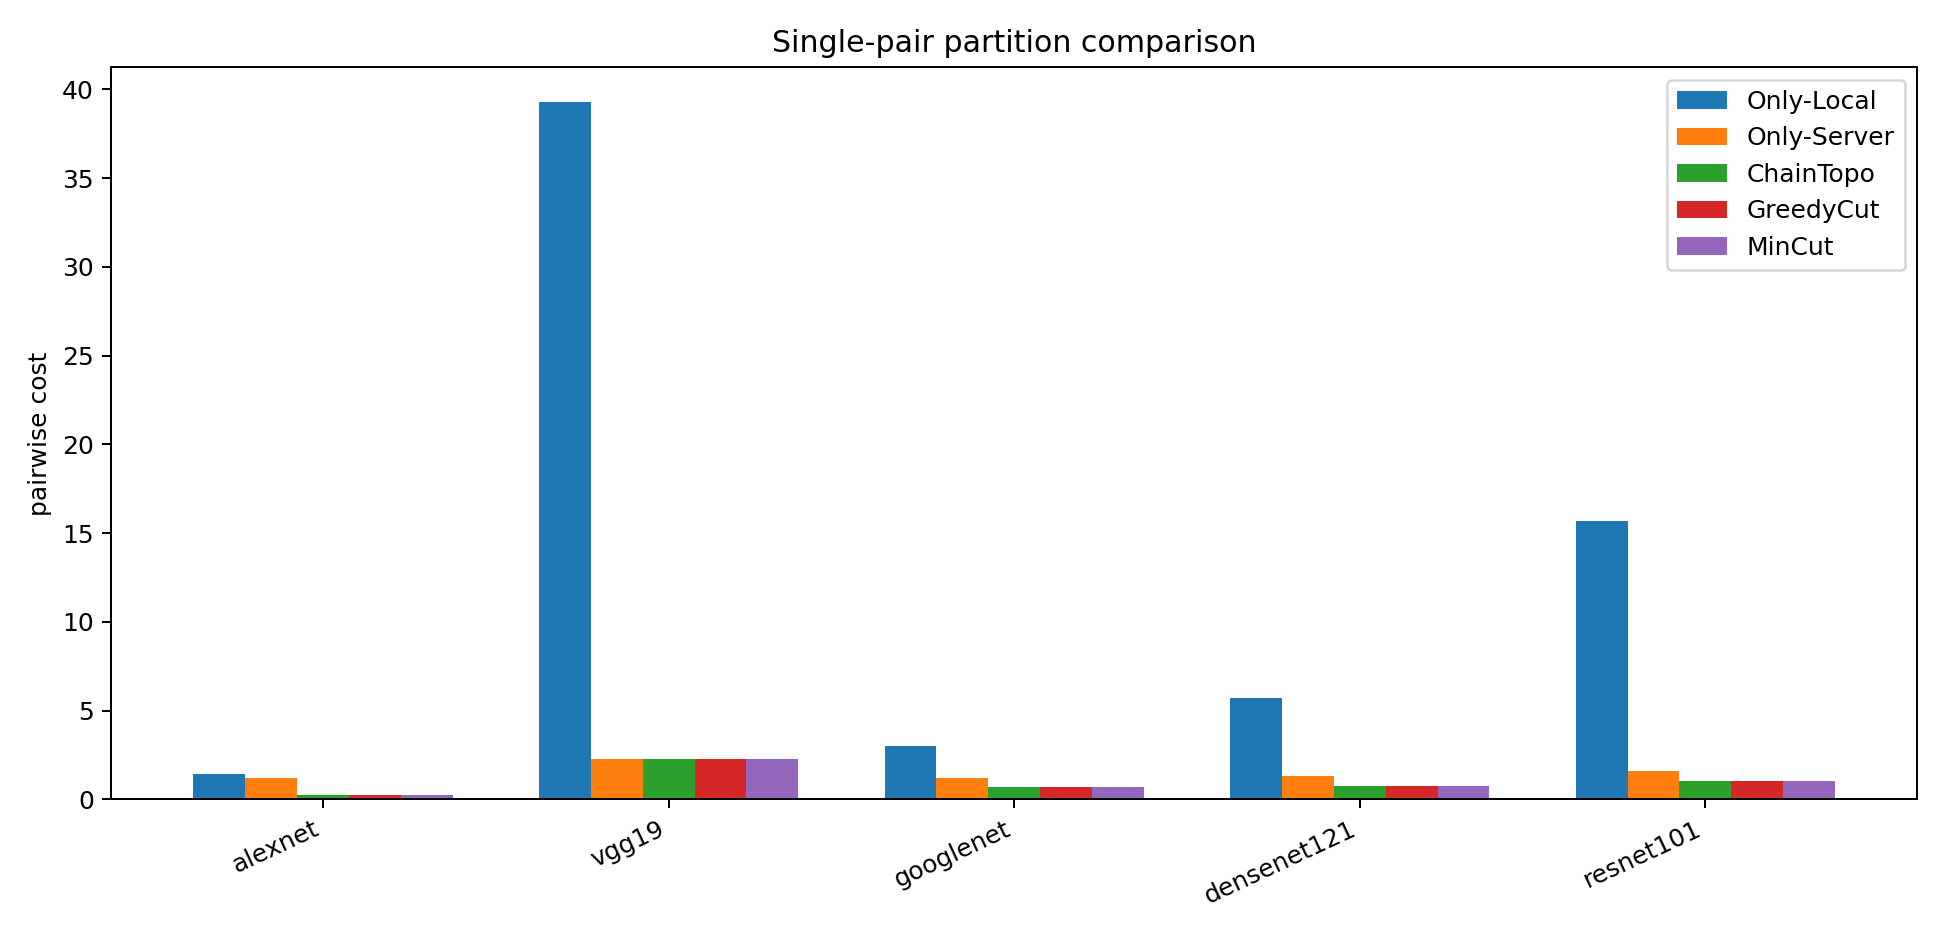
\includegraphics[width=0.98\linewidth]{outputs_mixed5_ratio4_midonly/single_pair_cost.png}
\caption{Module-I standard single-pair comparison over the retained five-model set.}
\label{fig:singlepair}
\end{figure}

\subsection{Module I: Topology Stress on GoogLeNet}

The GoogLeNet stress case now shows a real structural advantage. The costs are:
\begin{itemize}
\item Only-Local: 9.0224,
\item Only-Server: 23.5706,
\item ChainTopo: 8.9252,
\item GreedyCut: 8.9252,
\item MinCut: 8.4123.
\end{itemize}

MinCut improves over ChainTopo and GreedyCut by 5.75\% and selects the
non-prefix multi-node cut
\texttt{inception4a\_branch1\_conv, inception4a\_branch2\_0\_conv,}
\texttt{inception4a\_branch3\_0\_conv, inception4a\_branch4\_1\_conv}.
This is the cleanest evidence in the current system that full DAG modeling can
matter numerically, not only conceptually.

\begin{figure}[t]
\centering
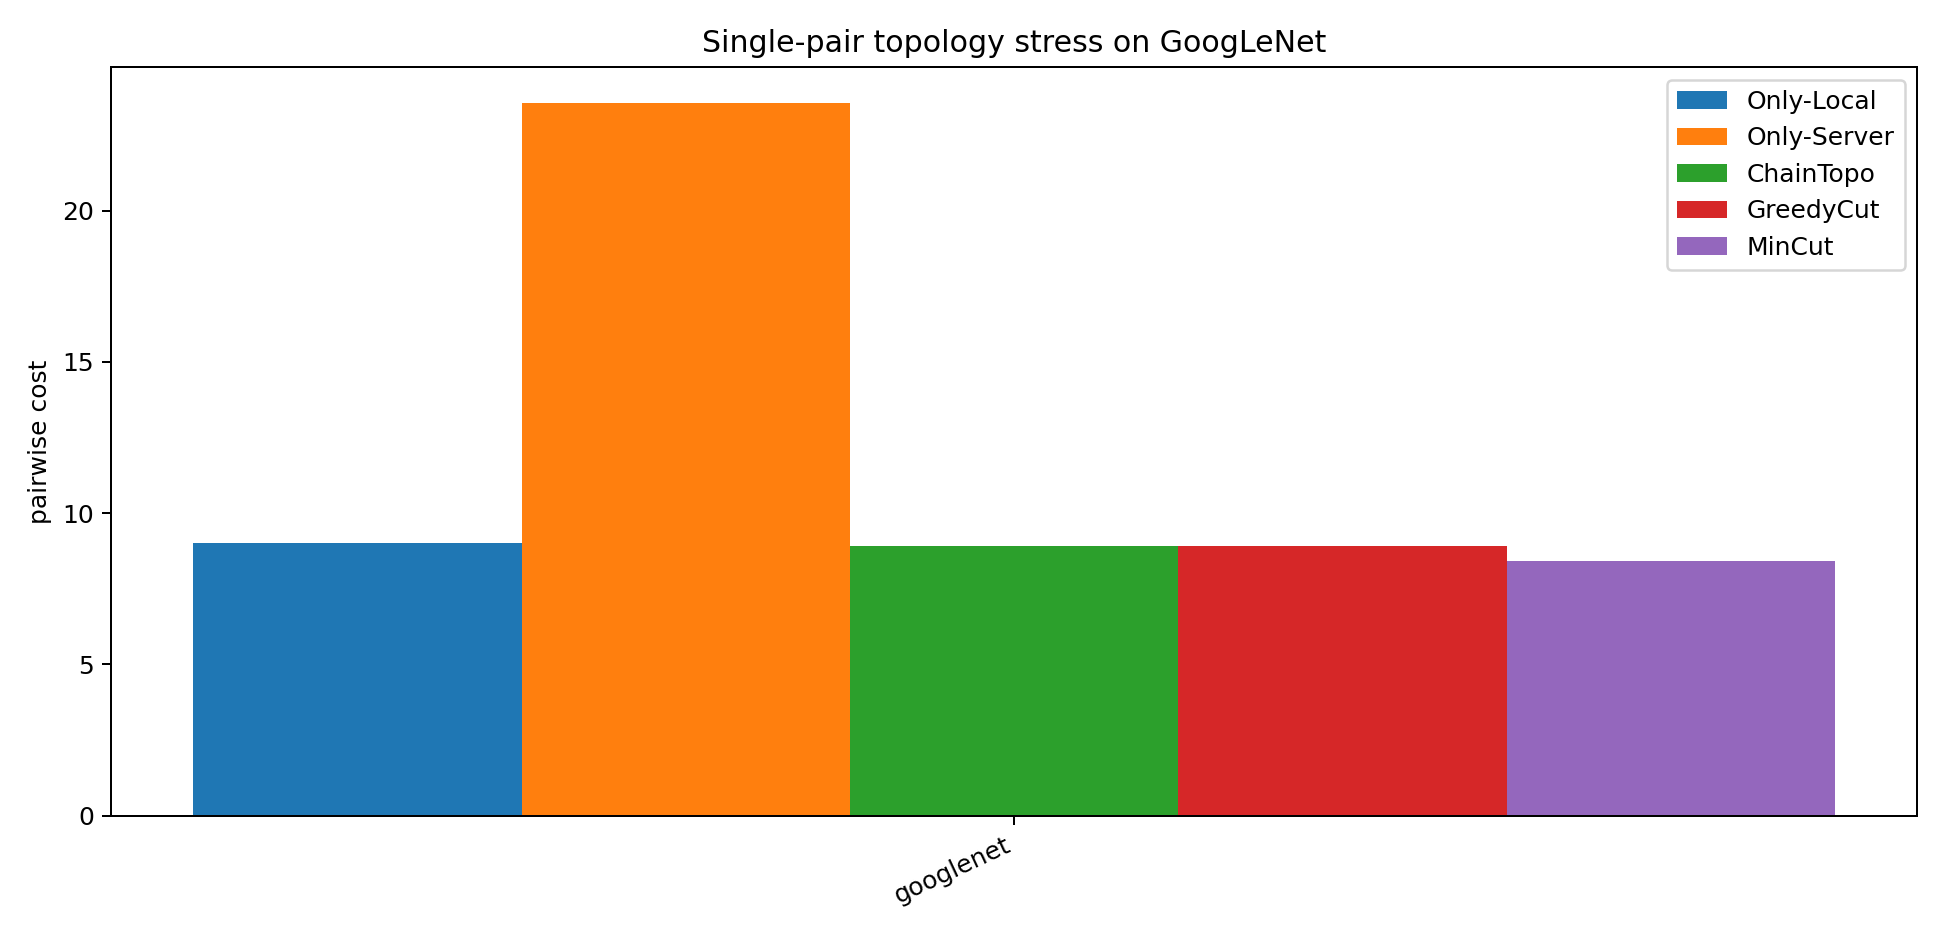
\includegraphics[width=0.9\linewidth]{outputs_mixed5_ratio4_midonly/single_pair_topology_stress.png}
\caption{Module-I topology-stress result on single-pair GoogLeNet.}
\label{fig:stress}
\end{figure}

\subsection{Module II: Unified Five-Model Mixed Scenario}

Table~\ref{tab:mixed5} reports the main multi-user result.

\begin{table}[t]
\centering
\caption{Results on the unified five-model mixed scenario}
\label{tab:mixed5}
\begin{tabular}{lccc}
\toprule
Method & Cost & Latency & Energy \\
\midrule
Only-Local & 108.7339 & 35.6403 & 73.0936 \\
Only-Server & 7.7255 & 4.8545 & 2.8711 \\
MinCut+BMatch & 5.5616 & 3.5217 & 2.0399 \\
MinCut+RMatch & 6.1054 $\pm$ 0.3213 & 4.0655 & 2.0399 \\
Rpartition+RMatch & 66.5244 $\pm$ 22.1488 & 23.2297 & 43.2947 \\
\bottomrule
\end{tabular}
\end{table}

MinCut+BMatch reduces total cost by 94.89\% over Only-Local, 28.01\% over
Only-Server, 8.91\% over MinCut+RMatch, and 91.64\% over Rpartition+RMatch.
This is the central system-level result: pairwise modeling quality still
matters even after matching enters the picture, and matching quality still
matters after pairwise partitioning has been solved well.

\begin{figure}[t]
\centering
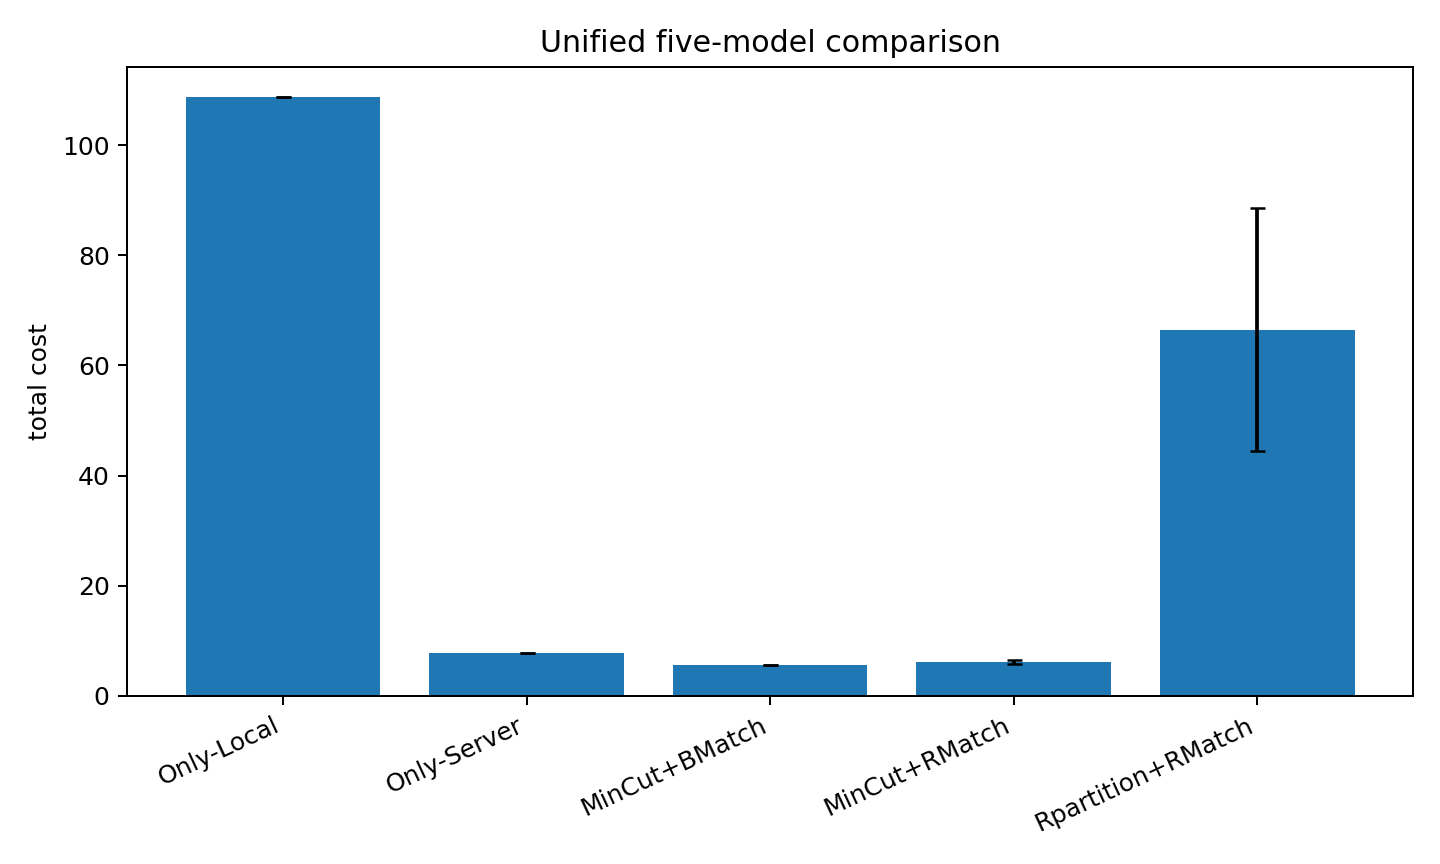
\includegraphics[width=0.92\linewidth]{outputs_mixed5_ratio4_midonly/mixed5_main_cost.png}
\caption{Module-II result on the unified five-model mixed scenario.}
\label{fig:mixed5-main}
\end{figure}

\subsection{Bandwidth and Energy-Weight Sensitivity}

Bandwidth sensitivity remains smooth. At 0.1 MB/s, MinCut+BMatch achieves
25.8757 while Only-Server reaches 59.4052. At 1 MB/s, the two methods are
5.5616 and 7.7255, respectively. At 5 MB/s, they become 2.9974 and 3.1318.
The selective upload model therefore still leaves meaningful room for
partitioning under constrained uplink bandwidth.

Beta sensitivity also remains smooth for $\beta$ from 0 to 4, indicating that
the framework preserves consistent behavior under different latency-energy
tradeoffs rather than depending on one specific weight choice.

\begin{figure}[t]
\centering
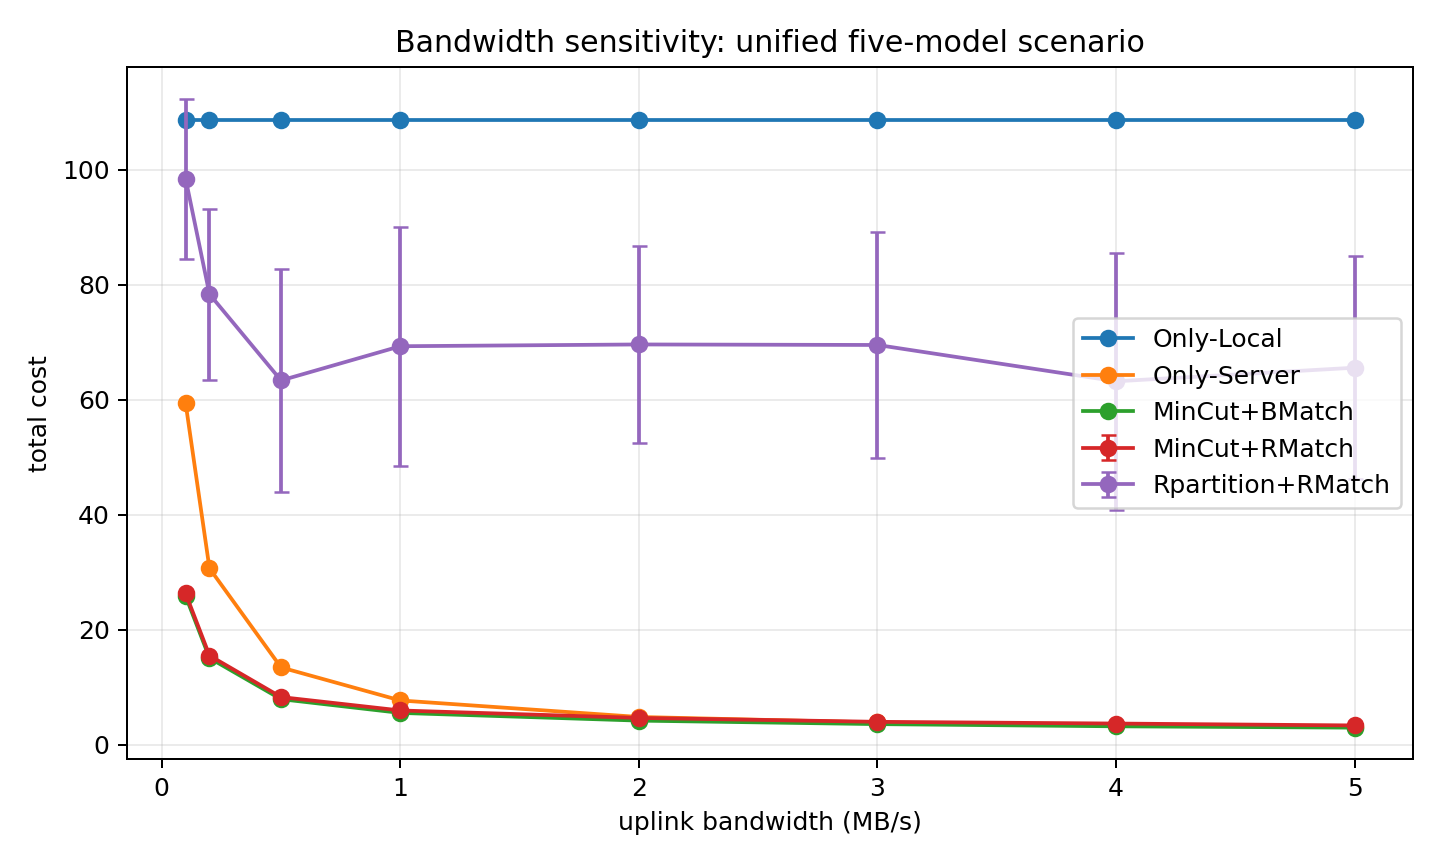
\includegraphics[width=0.92\linewidth]{outputs_mixed5_ratio4_midonly/mixed5_bandwidth_cost.png}
\caption{Bandwidth sensitivity on the unified five-model mixed scenario.}
\label{fig:bandwidth}
\end{figure}

\begin{figure}[t]
\centering

\includegraphics[width=0.92\linewidth]{outputs_mixed5_ratio4_midonly/mixed5_beta_cost.png}
\caption{Energy-weight sensitivity on the unified five-model mixed scenario.}
\label{fig:beta}
\end{figure}

\subsection{Online Extension: Slot-Wise Re-Optimization}

The online extension asks a narrower question than the static theory: once the
pairwise Min-Cut model is available, does slot-wise re-optimization help when
bandwidth, active users, and queue state vary over time?

In the bandwidth-trace scenario, Online MinCut+BMatch reduces average cost by
20.08\% over Static MinCut+BMatch and by 40.80\% over Online Only-Server,
while reducing average queue wait from 0.8644\,s to 0.4367\,s. In the
burst-load scenario, the online method reduces average cost by 20.93\% over
Static MinCut+BMatch and by 18.69\% over Online Only-Server. In the composite
non-stationary scenario, Online MinCut+BMatch achieves an average cost of
8.9200, compared with 10.2206 for Static MinCut+BMatch and 12.5794 for Online
Only-Server. The corresponding improvements are 12.73\% and 29.09\%,
respectively. The average queue wait drops from 0.9203\,s under the static
policy to 0.5052\,s under slot-wise re-optimization.

\begin{figure}[t]
\centering
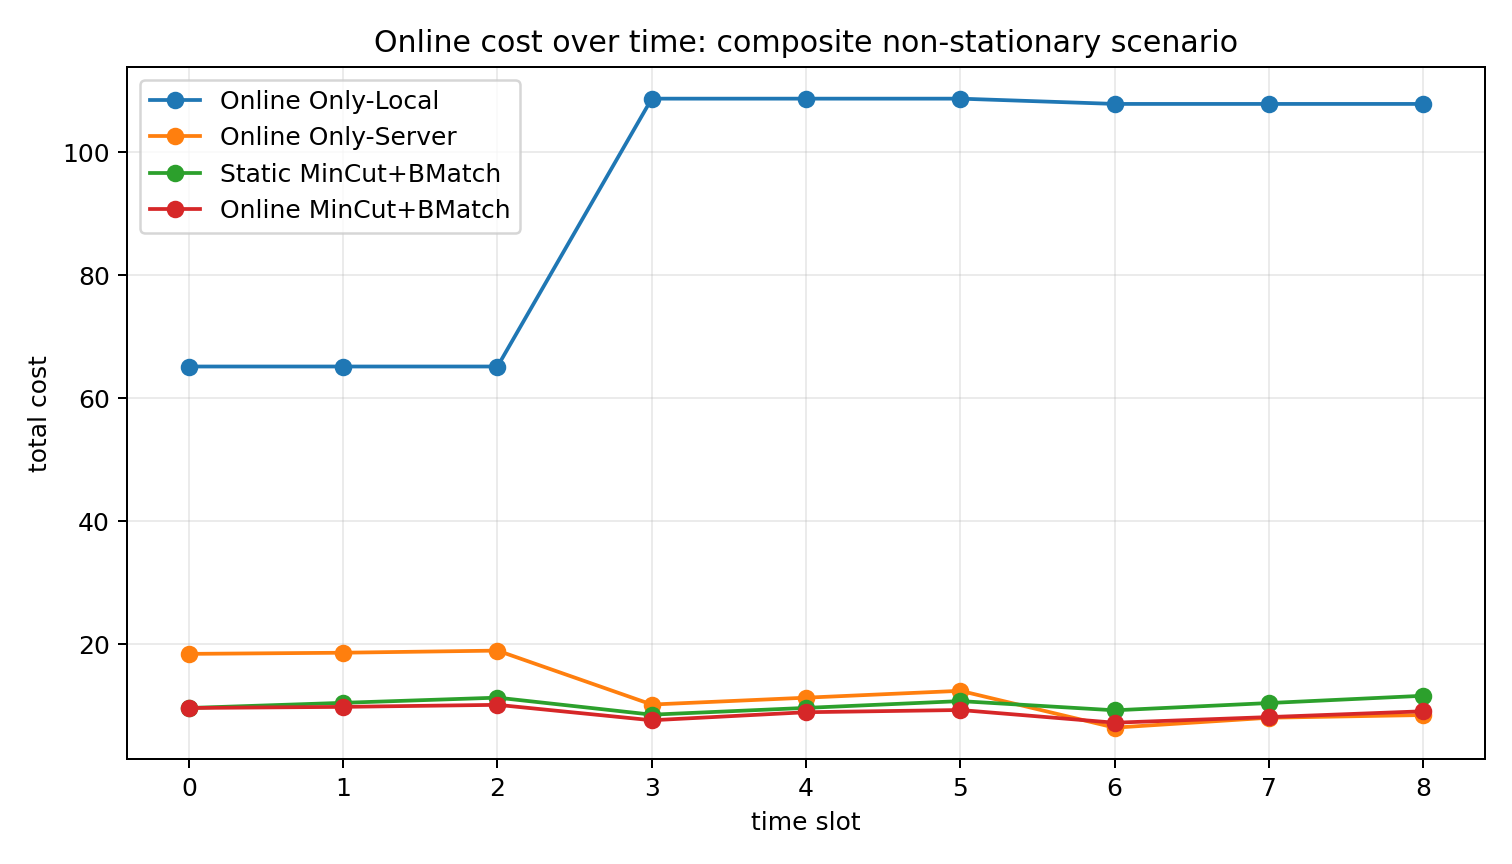
\includegraphics[width=0.92\linewidth]{outputs_mixed5_ratio4_midonly/online_cost_over_time.png}
\caption{Online composite non-stationary trace: total cost over time.}
\label{fig:online-cost}
\end{figure}

\begin{figure}[t]
\centering
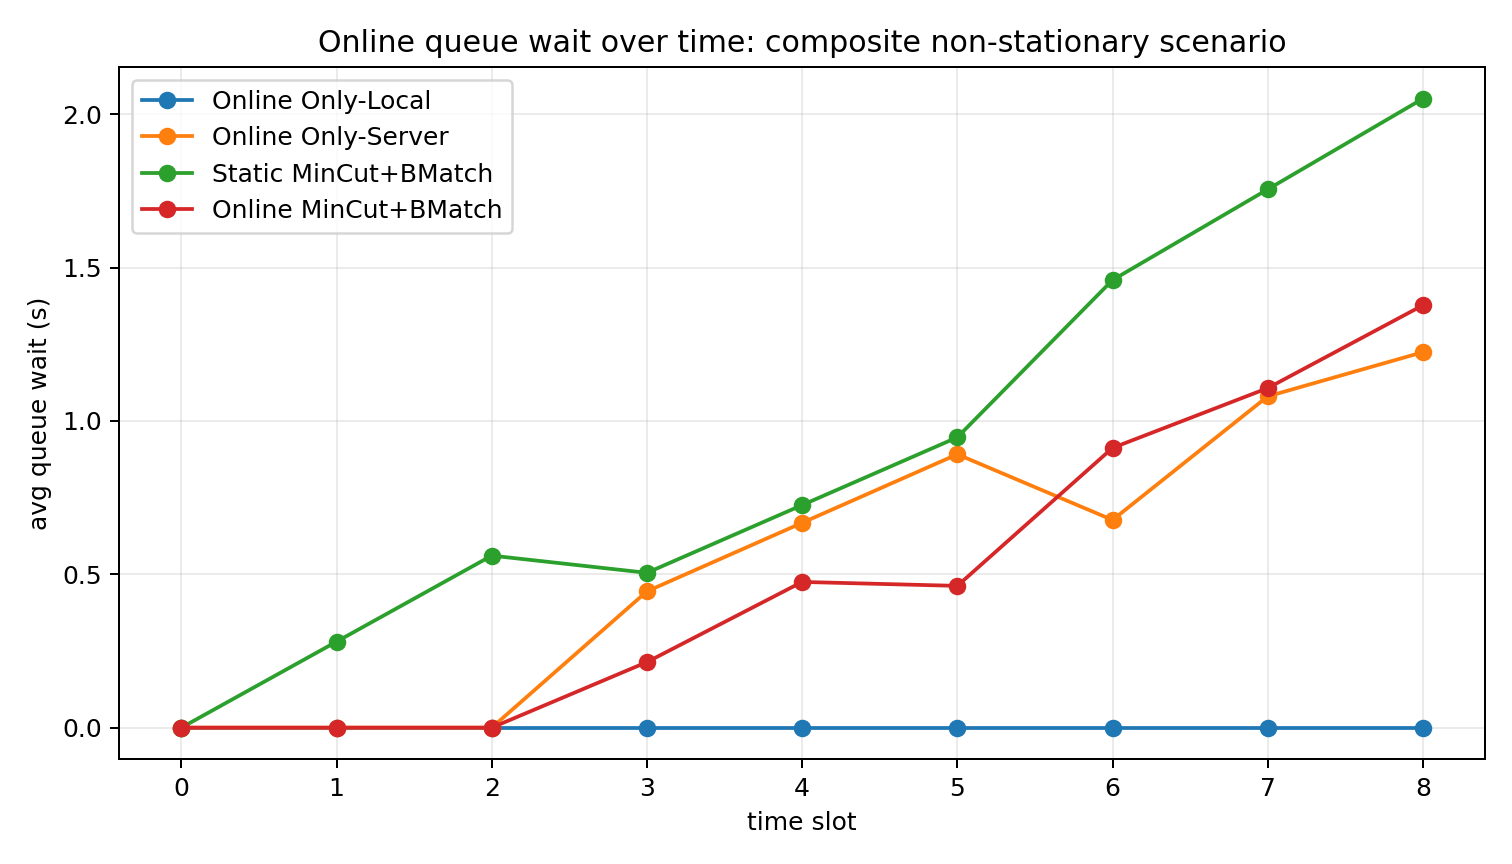
\includegraphics[width=0.92\linewidth]{outputs_mixed5_ratio4_midonly/online_queue_over_time.png}
\caption{Online composite non-stationary trace: average queue wait over time.}
\label{fig:online-queue}
\end{figure}

\subsection{Runtime and Scalability}

The runtime results show that MinCut remains efficient on the retained models:
\begin{itemize}
\item AlexNet: MinCut 0.70 ms, ChainTopo 0.65 ms, GreedyCut 0.74 ms;
\item VGG19: MinCut 1.11 ms, ChainTopo 2.43 ms, GreedyCut 2.92 ms;
\item GoogLeNet: MinCut 7.71 ms, ChainTopo 43.85 ms, GreedyCut 115.89 ms;
\item DenseNet121: MinCut 28.02 ms, ChainTopo 311.03 ms, GreedyCut 349.37 ms;
\item ResNet101: MinCut 53.26 ms, ChainTopo 126.04 ms, GreedyCut 158.77 ms.
\end{itemize}

In the 50-MD, 50-slot scalability case, cost-matrix construction takes
32747.86 ms while Hungarian matching takes 1.40 ms. The engineering bottleneck
is therefore the pairwise partition matrix construction, not the assignment
stage.

\begin{figure}[t]
\centering
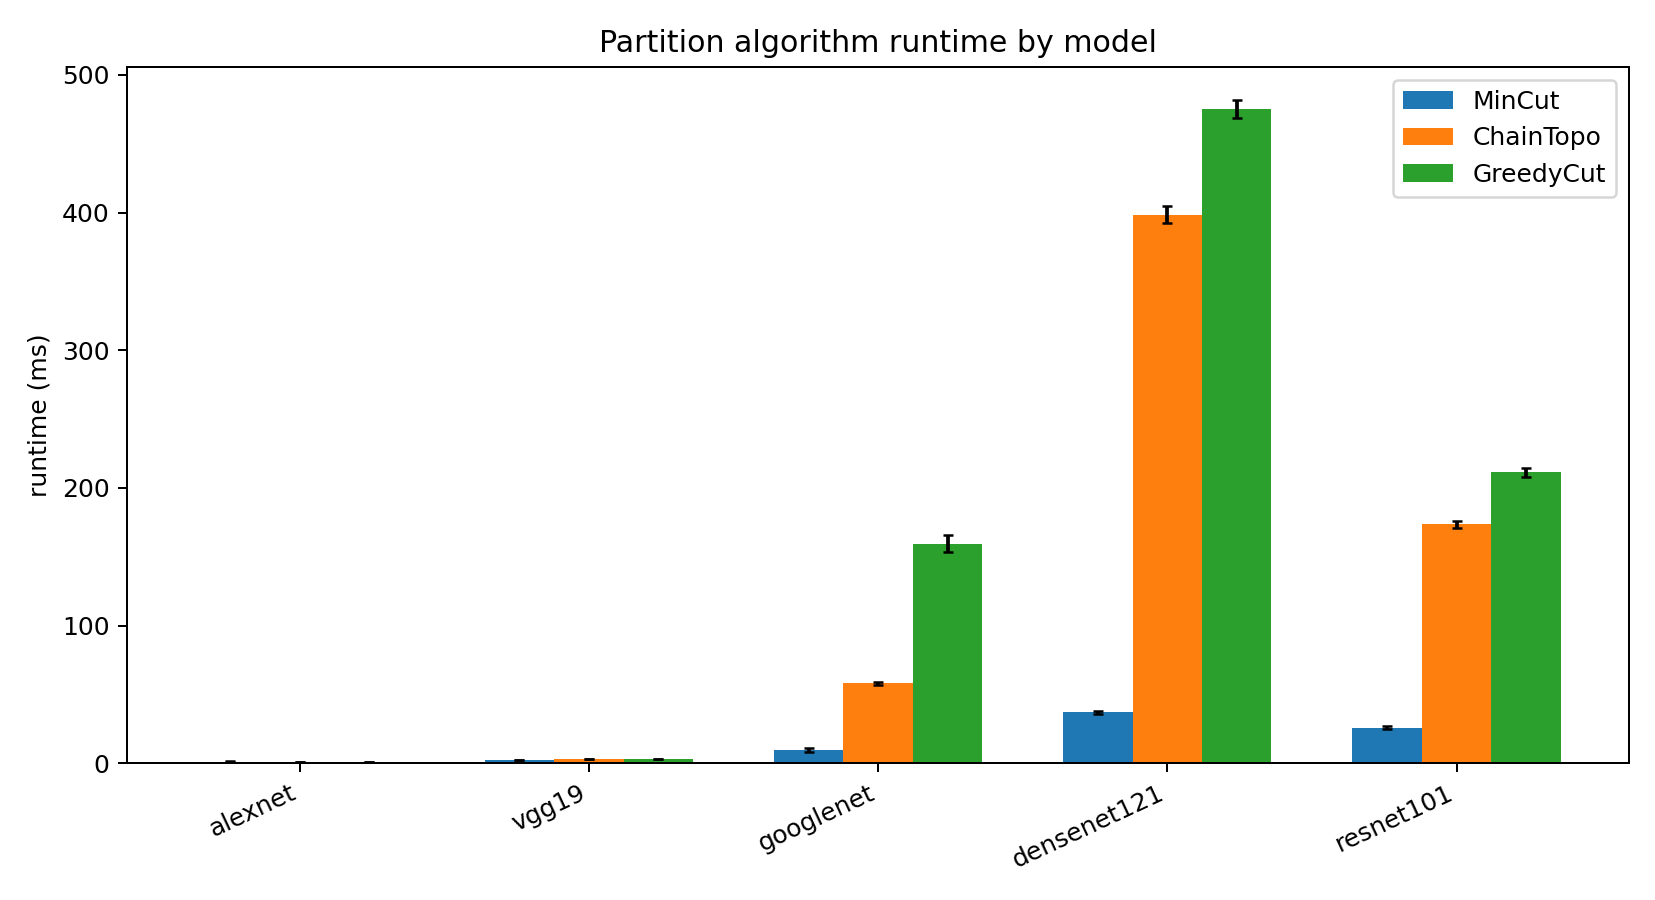
\includegraphics[width=0.92\linewidth]{outputs_mixed5_ratio4_midonly/algorithm_runtime.png}
\caption{Partition runtime by model.}
\label{fig:runtime}
\end{figure}

\begin{figure}[t]
\centering
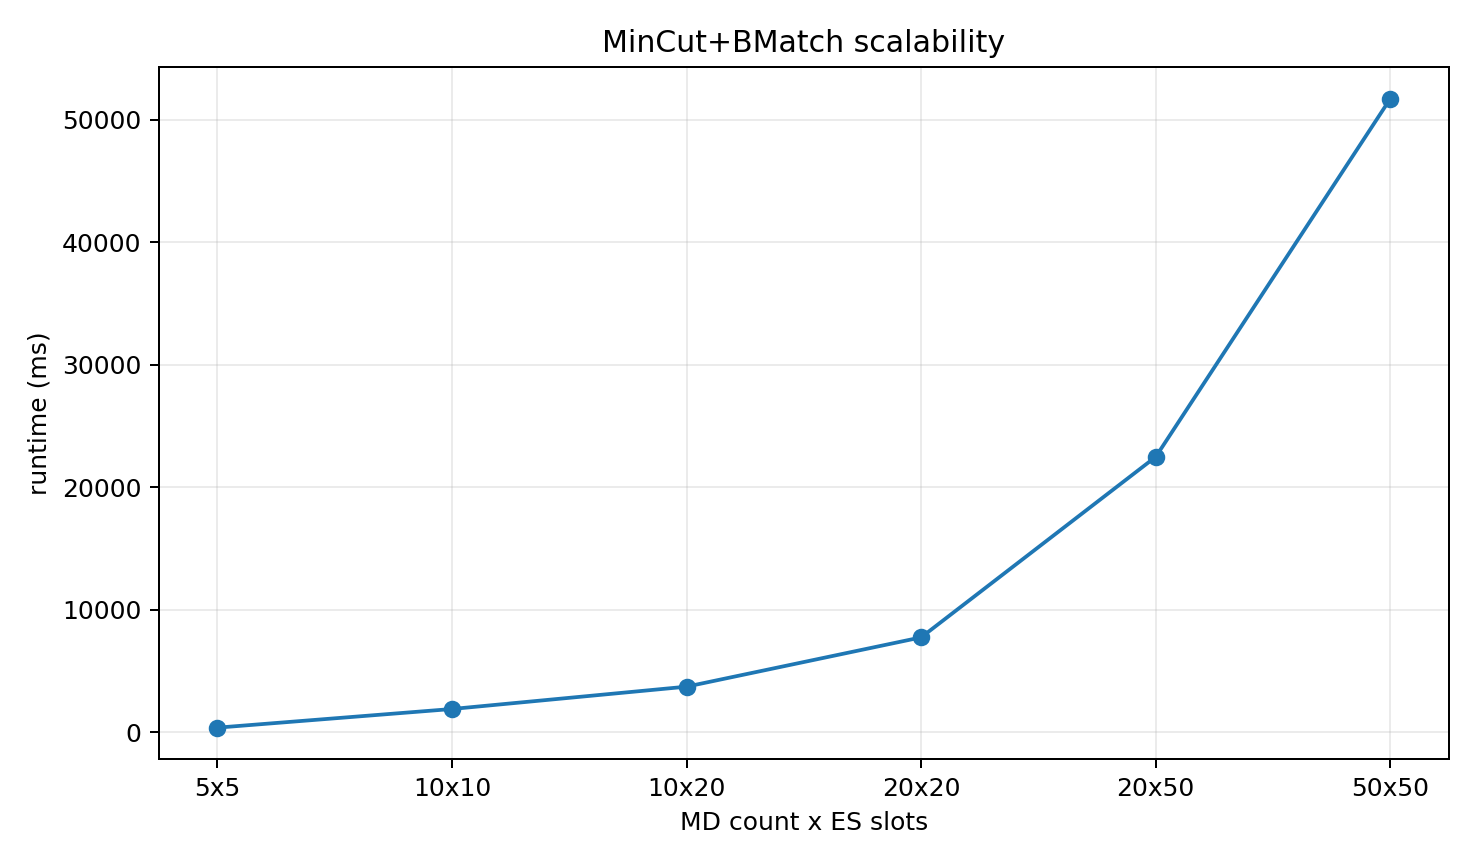
\includegraphics[width=0.92\linewidth]{outputs_mixed5_ratio4_midonly/scalability_runtime.png}
\caption{Scalability of MinCut+BMatch.}
\label{fig:scalability}
\end{figure}

\section{Discussion}

This work remains a simulation-driven algorithm paper rather than a full
end-to-end deployment paper. The ``global optimal'' statement applies only
under the independent \texttt{server\_slot} model. The online extension is
observation-driven slot-wise re-optimization; it does not claim
trajectory-wide optimality, competitive ratio, or Lyapunov-style guarantees.
The current results are also specific to the selective fixed-ratio upload
model. Compression latency, decompression latency, and compression-side energy
are deliberately ignored. These boundaries should remain explicit in the final
submission.

\section{Conclusion}

We reformulated collaborative DNN offloading into two static modules: globally
optimal DAG partitioning for each fixed MD-ES pair, followed by globally
optimal assignment over the resulting pairwise cost matrix. The current
five-model system shows that Min-Cut is never worse than strong chain baselines
in the standard single-pair setting, can reveal a real non-prefix structural
gain in the GoogLeNet stress case, and delivers clear system-level gains in the
unified mixed scenario. The same decomposition can also be reused as a
slot-wise adaptive controller under non-stationary bandwidth and queue
conditions.

\begin{thebibliography}{99}

\bibitem{joint}
Joint multi-user DNN partitioning and task offloading in mobile edge computing.

\bibitem{neurosurgeon}
Neurosurgeon.

\bibitem{dnnsurgery}
Dynamic adaptive DNN surgery for inference acceleration on the edge.

\bibitem{edgent}
Edgent and related collaborative intelligence systems.

\end{thebibliography}

\end{document}
